\documentclass{standalone}
\usepackage{tikz}
\usepackage{graphicx}

\begin{document}

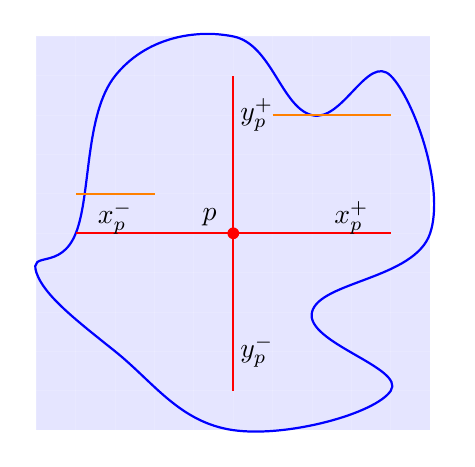
\begin{tikzpicture}

% Draw background pattern
\fill[blue!10] (-2.5,-2.5) rectangle (2.5,2.5);
\fill[white] (-2.5,-2.5) grid[step=0.5] (2.5,2.5);

% Define the poorly textured region shape
\draw[blue, thick] plot[smooth cycle, tension=0.7] coordinates {(-2,0) (-1.5,2) (0,2.5) (1,1.5) (2,2) (2.5,0) (1,-1) (2,-2) (0,-2.5) (-1.5,-1.5) (-2.5,-0.5)};

% Draw red lines for x_p and y_p
\draw[red, thick] (-2,0) -- (2,0);
\draw[red, thick] (0,-2) -- (0,2);

% Draw the orange error-causing pixels
\draw[orange, thick] (-2,0.5) -- (-1,0.5);
\draw[orange, thick] (0.5,1.5) -- (2,1.5);

% Draw the center point p
\node[circle, fill=red, inner sep=1.5pt] at (0,0) {};

% Label the points
\node at (-0.3,0.2) {$p$};
\node at (1.5,0.2) {$x_p^+$};
\node at (-1.5,0.2) {$x_p^-$};
\node at (0.3,1.5) {$y_p^+$};
\node at (0.3,-1.5) {$y_p^-$};

\end{tikzpicture}

\end{document}